\documentclass[11pt,a4paper,twoside,dutch]{report}
\usepackage[english]{babel}
\selectlanguage{english}

%%%%%%%%%%%%%%%%%%%%%%%%%%%%%%%%%%%%%%%%%%%%%%%%%%%%%%%%%%%%%%%%%%%%%%%%%%%%%
\newif\ifpublic \newif\iftwocol	% publication mode %
\newif\ifdraftmode \newif\ifdraftmode	% drafts mode %

%%%%%%%%%%%%%%%%%%%%%%%%%%%%%%%%%%%%%%%%%%%%%%%%%%%%%%%%%%%%%%%%%%%%%%%%%%%%%
% publishable version (no titlepage, credits, evaluation or attachments)%
%%%%%%%%%%%%%%%%%%%%%%%%%%%%%%%%%%%%%%%%%%%%%%%%%%%%%%%%%%%%%%%%%%%%%%%%%%%%%
%\publictrue	% 1-kolom publicatiemode (zonder %) of verslagmode (met %)
%\twocoltrue	% 2-kolommen publication mode
%\draftmodetrue	% 3-draft mode

%%%%%%%%%%%%%%%%%%%%%%%%%%%%%%%%%%%%%%%%%%%%%%%%%%%%%%%%%%%%%%%%%%%%%%%%%%%%%
% template packages en macro's %
%%%%%%%%%%%%%%%%%%%%%%%%%%%%%%%%%%%%%%%%%%%%%%%%%%%%%%%%%%%%%%%%%%%%%%%%%%%%% 
\ifpublic\iftwocol\twocolumn\fi\fi	% flag 1 or 2 columns %
\usepackage[utf8]{inputenc}
\usepackage{model}		% template %
\renewcommand{\redactie}[1]{\relax}	% nodig voor redactionele opmerkingen %

%%%%%%%%%%%%%%%%%%%%%%%%%%%%%%%%%%%%%%%%%%%%%%%%%%%%%%%%%%%%%%%%%%%%%%%%%%%%%
% packages %
%%%%%%%%%%%%%%%%%%%%%%%%%%%%%%%%%%%%%%%%%%%%%%%%%%%%%%%%%%%%%%%%%%%%%%%%%%%%%
\usepackage{algorithmic}
\usepackage{listings}
\usepackage[scaled]{helvet} %% Helvetica replica
\renewcommand*\familydefault{\sfdefault} %% Only if the base font of the document is to be sans serif
\usepackage[T1]{fontenc}


\begin{document}
\titelblad
	{Native Cross-platform Mobile Application Development}
	{W. de Kraker (0815283)} 
	{\INF}                     
	{\today}                  
	{Dhr. Y. S. Tjang}
	{Dhr. A. Chamani}

\ifpublic
	{\footnotesize{\input{samenvatting}}}
\else
	\pagenumbering{roman}
	\samenvatting

%lunatech aanhalen, aanleiding en concrete probleemstelling kort neerzetten. + thesis introduceren.


Nowadays mobile devices are vastly integrated into modern society. They bring us one step closer to satisfy our ever growing need to have information available anytime, anywhere. To help gain access to information on mobile devices we use so called \emph{apps}. 

However the fragmented nature of today's mobile ecosystem poses a challenge for mobile developers to develop apps which are suitable to run on all mobile devices \emph{(cross-platform}, since there is no de facto standard.

Currently there are several cross-platform mobile application development frameworks which offer a solution to this problem. 

Lunatech having expressed its interest in mobile app development, would like to know which of these framework, \emph{if any}, suits Lunatechs needs best. A research has been setup in order to resolve this question, its result is layed out in this thesis.



	\hoofdstuk{Credits}

It is still a bit to early to start thanking people. 
	\tableofcontents
	%\hoofdstuk{Defining the context}
The goal of this chapter is to define the context of the main research question.

\indent \emph{"How to develop a cross-platform mobile application while retaining the native look-and-feel?"}

\noindent Accordingly this chapter will define:
\begin{itemize}
\item the scope of \emph{cross-platform}
\item the concept of the \emph{native look-and-feel}
\end{itemize}

\paragraaf{Cross-platform}
This section will define the scope of \emph{cross-platform}. This will be done in two parts, first term platform will be defined after which will determined which platforms fall within the scope.

\subparagraaf{Platforms}
In order to determine which platforms should be supported for mobile development the following criteria have been provided by Lunatech:

\begin{enumerate}	
\item \emph{Platform type}\\
The platform has to be mobile, equipped with a touchscreen and support 3rd party applications. %Only smartphones will be targetted for development.
\item \emph{Platform marketshare}\\
The platform should have 10\% market share in the european continent.
\item \emph{Platform marketshare trend}\\
The market share trend from the past 6 months should not depict a trend directed below the set threshold of 10\% within the next 6 months.
\end{enumerate}

The platform type criteria is based on Lunatech's requirement to support smartphones and tablet computers. A smartphone can be defined as a smart phone is a next-generation, multifunctional cell phone that provides voice communication and text-messaging capabilities and facilitates data processing as well as enhanced wireless connectivity.\cite{Ni2006} Tablet computers, commonly referred to as tablet PCs, are wireless portable personal computers that utilize a touchscreen to access or process information.\cite{Leigh2011} The platform market share is the percentage per platform representing its share of the platforms market. Platform market share trend defined as the general course or prevailing tendency of the platforms market share. %TODO spellcheck. TODO: bron toevoegen http://dictionary.reference.com/browse/trend


%The smartphone only criteria implies that it is not a requirement to support support tablets and other mobile devices. This has significant influence on the marketshare criteria because it eliminates marketshare statistics based on operatingsystems, instead specific version details to be be included. %For instance this means that statistics which were harvested based on useragent strings have to be specifically scanned for \emph{iPhone} rather than \emph{Safai Mobile}.

\subparagraaf{Platform marketshares \& trend}
Platforms included in the cross-platform scope need to have a 10\% in share in the european smartphone market. 

There are several sources which provide statistical data over mobile platform market share. One of these is \emph{Net Market Share}. Net Market Share defines itself as the standard for tracking key internet technology usage market share. This means their statistical data is usage based, because it is aggregated from tracking users on the internet. Net market share aggregates its data from over 40,000 websites with approximately 160 million visitors per month.\cite{NetApplications2012}


An alternate source for market share data is \emph{Gartner}. Gartner describes itself as being the world's leading information technology research and advisory company.\cite{Gartner2012} In an annual publication Gartner publishes a smartphone market share report. In contrast to Net Market Share this report has been based on manufacture unit sales data. Although very accurate, it does not reflect real usage nor is it an up to date source, i.e. the latest publication dates from august 2011.\cite{Pettey2011} Therefore Net Market Share is favorable over Gartner.


\begin{centering}
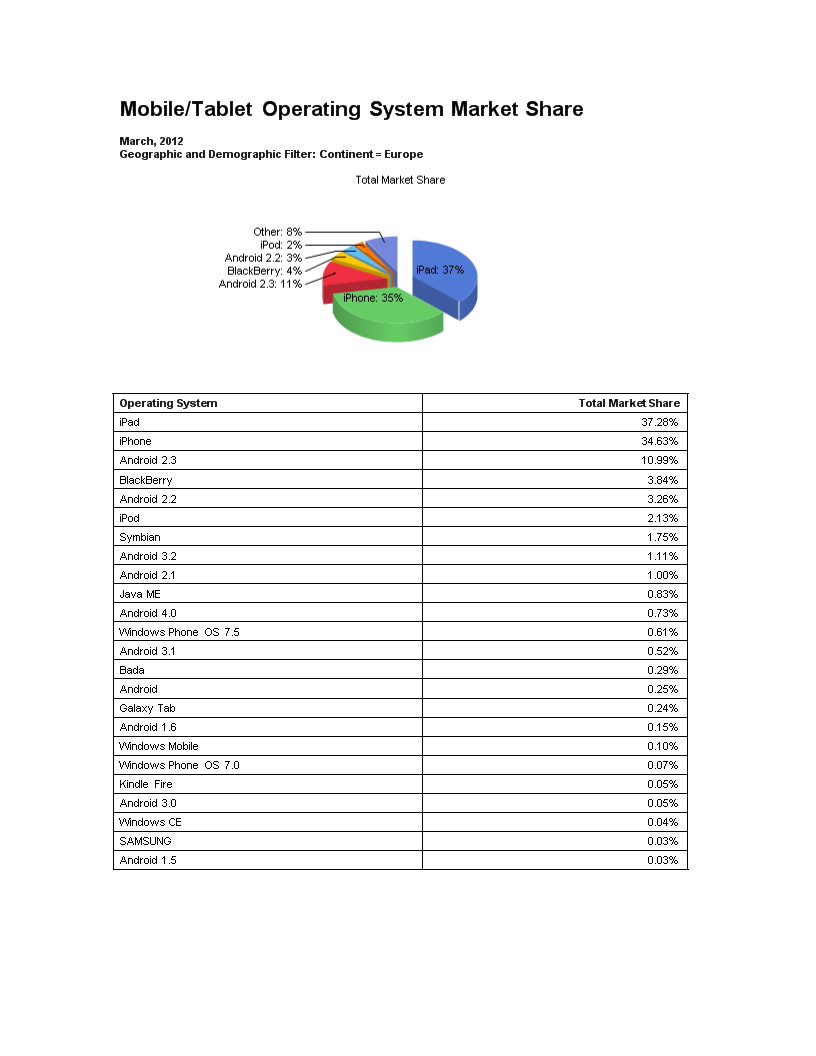
\includegraphics[scale=0.5]{images/netmarketshare_march2012.png}\\
\end{centering}

% \begin{tabel}{|>\R p{\Procent{25}} | >\R p{\Procent{25}} |}{vbx}{Marketshare in the european continent as of march 2012\cite{Netmarketshare2012}}
% \hline
% \bf{Operating System} & \bf{Total \% Market Share}\\
% \hline \hline
% iOS & 74.04\\
% Android & 18.36\\
% BlackBerry & 3.84\\
% Symbian & 1.75\\
% Java ME & 0.83\\
% Windows Phone & 0.68\\
% Bada & 0.29\\
% Windows Mobile & 0.14\\
% Kindle & 0.05\\
% Samsung & 0.03\\
% LG & 0.01\\
% ZTE & 0.00\\
% Palm & 0.00\\
% \hline
% \end{tabel}

% \begin{centering}
% 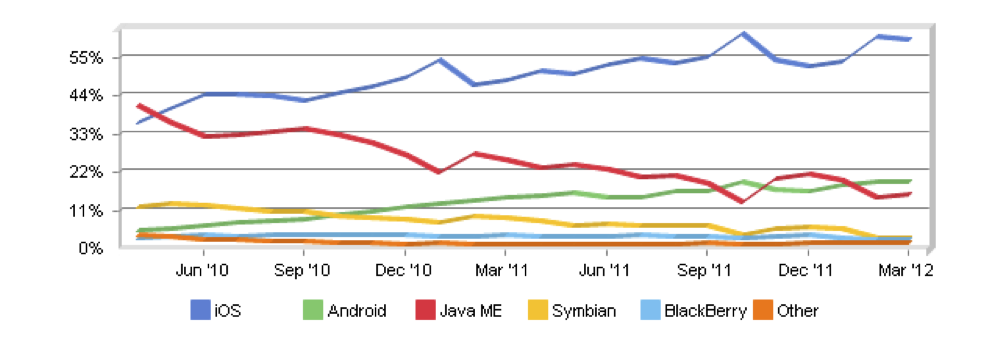
\includegraphics[scale=0.6]{images/marketsharetrendsApril10Tomay12.png}\\{World wide mobile OS Marketshare trends, April 2010 up to may 2012}\\
% \end{centering}

\begin{tabel}{|>\R p{\Procent{25}} | >\R p{\Procent{25}} |>\R p{\Procent{25}} |}{vbx}{Market share in the european continent as of October 2011 and March 2012\cite{Netmarketshare2012}}
\hline
\bf{Operating System} & \bf{Market Share in October 2011} & \bf{Market Share in March 2012}\\
\hline \hline
iOS & 75.78 & 74.04\\
Android & 16.14 & 18.36\\
BlackBerry & 3.56 & 3.84\\
Symbian & 2.69 & 1.75\\
Java ME & 0.87 & 0.83\\
Windows Phone & 0.27 & 0.68\\
Bada & 0.35 & 0.29\\
Windows Mobile & 0.27 & 0.14\\
Kindle & 0.00 & 0.05\\
Samsung & 0.06 & 0.03\\
LG & 0.01 & 0.01\\
\hline
\end{tabel}

iOS and Android both cover over 10 \% of the market, together they are good for 92.40 \% of the total mobile market as of march 2012 in the european continent.


% dit lijkt weg te kunnen:
% There are serveral sources for statistics relating to mobile platform marketshare. Although each based on their own source for gathering statisical data, there are generally 3 ways to collect such data:
% \begin{enumerate}
% \item \emph{Interview based}\\
% A market survey based on data gathered from (public) interviews.
% \item \emph{Sales based}\\
% A market survey based on the calculations from manufactorer sales data.
% \item \emph{Usage probing}\\
% A market survey where the device specific properties are measured to collect data.
% \end{enumerate}

% An interview based method of gathering does relies on the following algorithm provide an realistic image:

% A sales based does not j therefor i. Therefor method based on usage probing is favorable.
% Netmarketshare is a company which provides statistcs based on the usage probing method. It does this by collecting data from the useragent string. This is a piece of information a browser (and thus the device)\footnote{Although the useragent string is manipulatable we neglect this possibility} identifies itself with.



\subparagraaf{Platform versions}
In order to determine which versions per platform will be supported Lunatech has stated that a version must have at least a 10\% user share of the platform. 

\noindent For Android this means the versions:
\begin{itemize}
\item 2.2 - \emph{Froyo} (19.1\%)
\item 2.3.3 to 2.3.7 - \emph{Gingerbread} (64.6\%)
\end{itemize}
This statement is based on data gathered by the number of Android devices that have accessed Google Play within a 14-day period ending on the data collection date noted below.
\begin{centering}
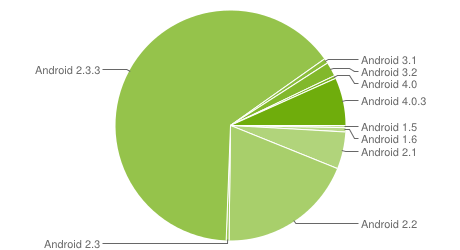
\includegraphics[scale=0.35]{images/androidversionchart.png}\\{Android platform version distribution, as of June 1st, 2012.\cite{GoogleAndroid2012}}\\
\end{centering}

\noindent For iOS this includes the versions:
\begin{itemize}
\item 4.3 (15.0\%)
\item 5.1 (84.0\%)
\end{itemize}
\begin{centering}
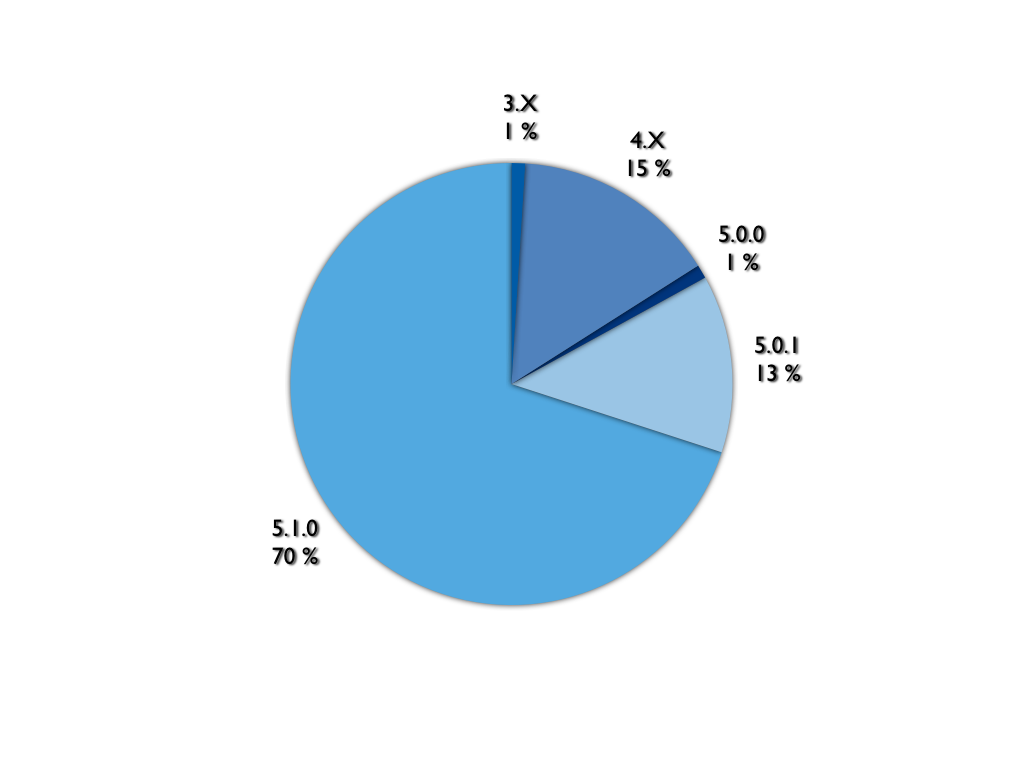
\includegraphics[scale=0.35]{images/iosversionchart.png}\\{iOS platform version distribution, as of May 26th, 2012.\cite{Sylvain2012}}\\
\end{centering}



\subparagraaf{Conclusion}
Apple iOS and Google Android both adhere to the criteria set by Lunatech and will be included in the scope of cross-platform. In conclusion \emph{cross-platform} support is defined as compatible to run on iOS 4.3 or greater and Android 2.2 or greater.


\paragraaf{Native mobile applications}
This paragraph will define the paradigm of \emph{native look-and-feel}. 

A native application is an application inherent to the platform for which it was built using techniques proprietary to the platform. For example, an iOS application is native when written in Objective-C and an Android application is written in Java.  Native applications are typically fast and can access the device's native API's.

\subparagraaf{The native look-and-feel}
When written in the native framework for a platform a mobile application receives access to the available public libraries of the platform. These libraries include those which provide the developer with a pre-fabricated set of user interface components. These can be seen as the building blocks for the graphical user interface on that platform. When used, the general style of the mobile application gains constancy to the overall user interface design of the platforms operating system. This gives an application its native look, which in turn participates to the \emph{native feel}.

%with a feeling of recognition when using the application, userinterface elements work as they expected based upon experience with using the operating system.
%todo: add some notes about the Human Interface Guidelines.

The \emph{native feel} of a mobile application can be defined as the speed in which the user interface elements, the responsiveness of user interface elements to touch events, and smoothness of the animation in which the user interface elements are moved. A native mobile application has the advantage of hardware acceleration. This means its code has been precompiled and directly executed by the device CPU, rather than having to be interpreted by the device's browser. As a result of this the user interface elements are rendered faster and it \emph{feels} smooth.


\paragraaf{Alternative mobile application types}
\subparagraaf{Web applications}
A mobile web application is an application developed with web technologies such as JavaScript and HTML with CSS. It is in fact nothing more than a website designed to fit on a mobile device's display, often they resemble the style of a native application rather than a traditional website. These applications are built with a JavaScript library to add support for scrolling and handling events. Touch events are handled via user interface elements provided by the library. Examples of these libraries include jQtouch, SenchaTouch

% todo: screenshots/links neerzetten.

\subparagraaf{Hybrid applications}
A hybrid application in mobile development refers to an application which use a native shell wrapped around web app. There are generally two forms of native shells, the first is a \emph{webview} and the second a native framework which exposes an JavaScript API to provide the web application access to otherwise native API's.
%TODO framework example.

{\bf Webview-based hybrid applications}\\
A web-view based hybrid application is a web based mobile application wrapped in a web-view. A web-view is a view or element which acts like a browser would, e.g. it is able to render HTML and run javascript.  It is readily available in the native libraries. The advantage of a web-view based hybrid application over an normal web application is that it can be published via the devices native application publishing platforms, i.e. a web-view based hybrid application targeted for the iPhone can be placed in the Apple Appstore. 

Worklight is an example of a framework which can be used to develop web-view based hybrid applications.

{\bf Framework hybrid applications}\\
A Framework based hybrid application is a web-view based application built upon a framework which provides an API to allow the application access to otherwise native API's. The framework is written in the platforms native programming language making it possible to access the native API, such as reading contact list, composing of text messages, full access to the location API, etc.

PhoneGap is an example of a framework which can be used to develop mixed hybrid applications.

\paragraaf{Comparison}
Web applications are quick and cheap to develop. Written entirely in HTML, CSS and JavaScript. Executed by the mobile
browser and therefore cross - platform by default, but less powerful than native apps.
 
Hybrid Applications (Web), the app's source code consists of web code executed within a native wrapper that is provided by a framework.
 
Hybrid Applications (Mix), the developer augments the web code with a Javascript API to create unique features and
access native APIs that are not yet available via the browser, such as AR, NFC and others.
 
Native Application are platform-specific. Requires unique expertise and knowledge. Pricey and time consuming to develop but
 delivers the highest user experience of all approaches.

\begin{centering}
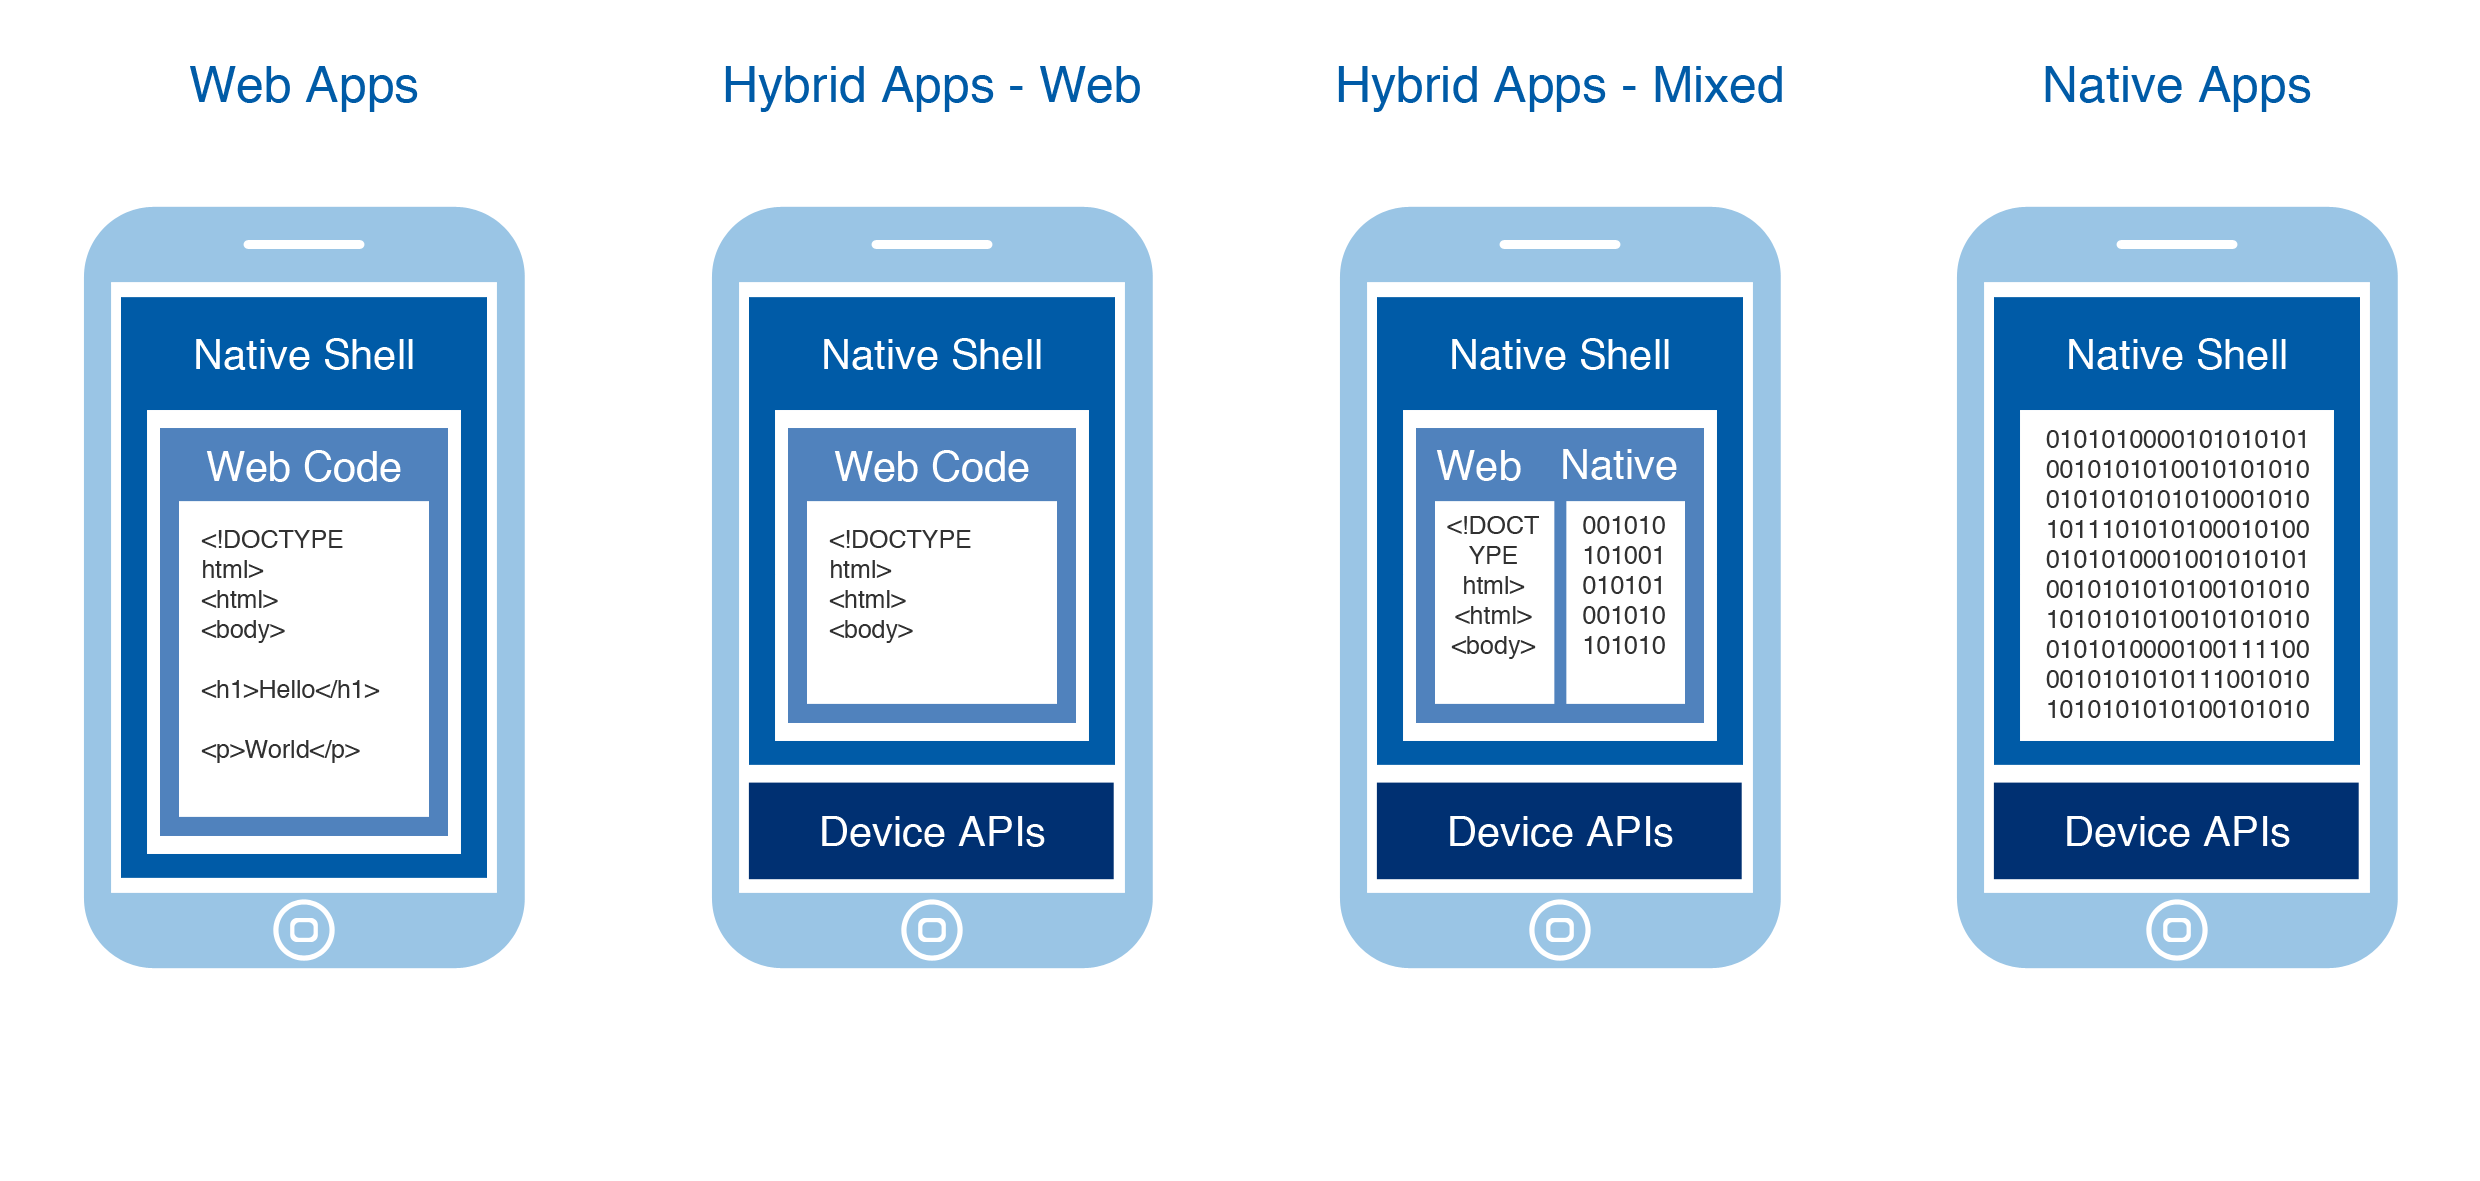
\includegraphics[scale=0.5]{images/apptypesdefined.png}\\{Different types of mobile applications\cite{IBM-Worklight2012}}\\
\end{centering}

\paragraaf{Conclusion}
A natively written mobile application provides the user with an experience immersed to that of the level of the device's operating system. This is due to two reasons:
\begin{itemize}
\item
\emph{Performance}\\
a native application is faster because it has direct access to memory and CPU
\item \emph{Looks}\\
a native application looks and feels more coherent to the device's operating system because it is able to make use the of the provided user interface elements.
\end{itemize}
	\pagenumbering{arabic}
\fi
	\hoofdstuk{Introduction}

\paragraaf{Problem statement}

Lunatech has demand for the development of cross-platform mobile applications. Currently these applications are been developed using webtechnologies such as HTML5 and Javascript. A mobile application developed this way is refered to as webapp because it runs in a browserbased environment and is often hosted at a webserver rather than downloaded to the device itself.
%\footnote{Note: when mentioning the word 'current', it refers to the old situation as the process to get to the actual current situation is being illustrated}

The problem with webapps is that they lack in user experience. This is mainly due manner in which user interface components are build in HTML. Every platform has its own set of recognizable elements, but these cannot be accessed from within the browser environment. As a result of this the app will feel dislocated to the user because it's style doesn't match the rest of the platform. It tries to look and feels native, but never gets arround the fact that it's a webapp.

The direct alternative to webapps are native apps, native are writting using technologies proprietary to each platform, hench the term 'native'. What these applications lose in terms of cross-platform support they make up in terms of user experience.  A native app has acces to all the platforms propietary libraries and can rely on the user interface elements provided through these libraries.

Lunatech would like to know how to make use of the look-and-feel from native apps with the cross-platform support of webapps.

\paragraaf{Research questions}

Main research question:
\begin{itemize}
\item \emph{How to develop a cross-platform mobile application while retaining the native look-and-feel?}
\end{itemize}

\noindent Sub research questions:
\begin{itemize}
% \item \emph{Which mobile platforms should be targetted for cross-platform mobile application development?}
% \item \emph{How is the native look-and-feel defined?}
\item \emph{Is it viable to implement my own solution to cross-platform mobile application development?}
\item \emph{Which solutions to cross-platform mobile application development currently exist?}
\item \emph{Which of these solutions offer the defined native look-and-feel?}
\item \emph{Is this solution viable for commerical useage?}
\end{itemize}

\paragraaf{Research method}


First the \emph{native look-and-feel} needs to be defined. After which it's nessecary to define the scope of \emph{cross-platform} by determining which platforms should be targetted.

Once the variables in main research question are fully defined the possiblity to look for existing solutions opens up. During a preliminary research a market survey will have to be performed in order to deterime which solutions to cross-platform app development are available on todays market. Each found solution will be given a closer look and categorized based on requirements provided by Lunatech. Once the categorization is complete the solutions will be filtered based on how far the requirements have been met.

A comparisson test will be performed in order to determine which solution meets is potentially viable for commercial use by Lunatech. This test will consist of a short analysis per solution based on by Lunatech criteria, and a practical part where a benchmark application will be built. The results will be compared and the solution which offers the most complete set of features will be deemed potentially viable for commercial use by Lunatech.

This alone however is not enough to answer the main research question. To determine if the chosen solution is viable for commercial use by Lunatech a case study will be performed based on a realistic scenario Lunatech might encounter. During this case study the solution will be analysed and evaluated.

The results of the case study and the analysis will participate to answering how to develop a cross-platform mobile application while retaining the native look-and-feel. In addition to answering the main research question an recommendation will be given to Lunatech regarding the possible adoptation of the solution for commercial usage.




%todo methode verantwoording.
\newpage
\begin{centering}
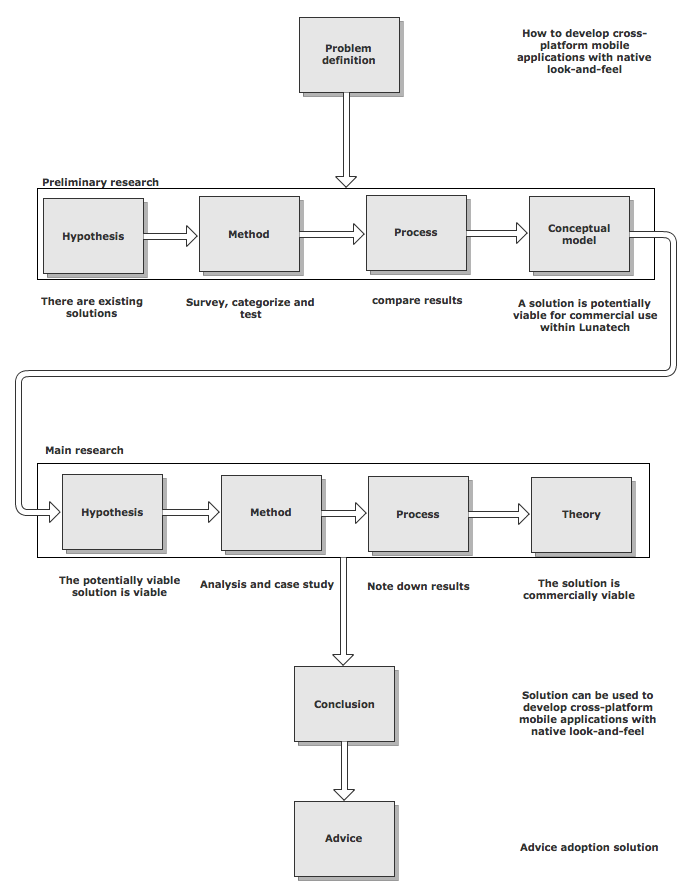
\includegraphics[scale=0.6]{images/researchprocess.png}\\{Research method diagram}\\
\end{centering}

%verantwoorden: why it works analysis. + verantwoorden niet naar andere oplossingen kijken.


	\hoofdstuk{Background}
\paragraaf{Lunatech Research B.V}
Lunatech provides application development services, completely based on open-source web and Java technologies and open standards. They are early adopters of new technology, and use cutting-edge frameworks and tools. To stay up-to-date, their developers have the opportunity to research, try new technologies and contribute to open-source projects. The company consists mainly of software developers. Everyone (except the director) writes code, on top of which some staff have a secondary management role, and the staff who will deliver a project interact with the customer directly.

\paragraaf{Rotterdam University of Applied Sciences (Hogeschool Rotterdam)}
Rotterdam University is one of the major Universities of Applied Sciences in the Netherlands. Currently almost 30,000 students are working on their professional future at the university.
The university is divided into eleven schools, offering more than 80 graduate and undergraduate programmes in seven fields: art, technology, media and information technology, health, behaviour and society, engineering, education, and of course, business.\cite{HogeschoolRotterdam2012}

\paragraaf{Student no. 0815283}
%TODO: zinvolle achtergrond informatie over mezelf toevoegen.
Student no. 0815283 is a 4th year computer sceince student at the Rotterdam University of Applied Sciences. Student no. 0815283 has a passion for things that are open source or have a sexy Apple logo on it. With over 2 years (professional) experience in mobile development he is the man for the job.
	\hoofdstuk{Mobile platforms}



\paragraaf{Introduction}
% per platform: van wie is het, wat is de geschiedenis, waar wordt het gebruikt, welke achterliggende techniek drijft het?
% plaatjes homescreens of devices toevoegen, visueel maken.

In order to define which mobile platforms should be targeted for cross-platform mobile application development the following chapter presents a concise overview of:

\begin{itemize}
\item
the current mobile operating systems for mobile platforms, with in smartphones specific. 
\item
the current market share and trends
\end{itemize}

In this thesis \emph{mobile platforms} encapsulate only smartphones as it has not been a requirement to support tablets and other mobile devices.

A smartphone can be defined as a smart phone is a next-generation, multifunctional cell phone that provides voice communication and text-messaging capabilities and facilitates data processing as well as enhanced wireless connectivity.\cite{Ni2006}



\subparagraaf{Apple iOS}
iOS is a proprietary mobile operating system, developed by Apple Inc. It was originally released in 2007 for the iPhone and iPod Touch. iOS also became the main operating system of the iPad and Apple TV.

\begin{centering}
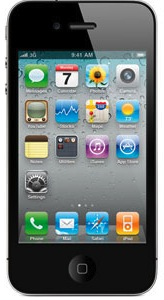
\includegraphics[scale=0.5]{images/iphone4.jpg}\\{4th generation Apple iPhone running iOS 4}\\
\end{centering}


\subparagraaf{Google Android}
Android is a open source mobile operating system, developed by the Open Handset Alliance, led by Google and other companies.\cite{Inc.2012}

\begin{centering}
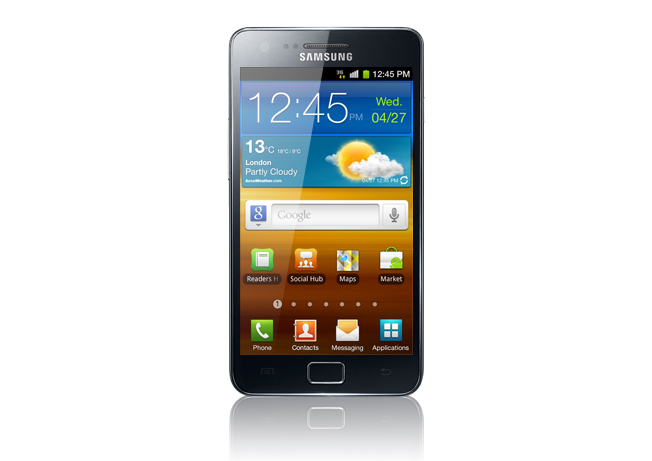
\includegraphics[scale=0.35]{images/android_sgs2.jpg}\\{Samsung Galaxy S2 running Android 2.3}\\
\end{centering}


\subparagraaf{BlackBerry OS}
BlackBerry OS is a proprietary mobile operating system, developed by RIM\emph{(Research In Motion)} for its line of BlackBerry mobile devices.

\begin{centering}
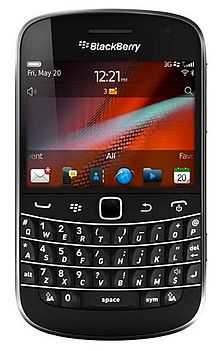
\includegraphics[scale=0.5]{images/Blackberrybold9900.jpg}\\{BlackBerry Bold 9900 running BlackBerry OS 7.1}\\
\end{centering}


\subparagraaf{Windows Phone 7}
Windows Phone 7 is a mobile operating system developed by Microsoft as a successor to its Windows Mobile platform.

\begin{centering}
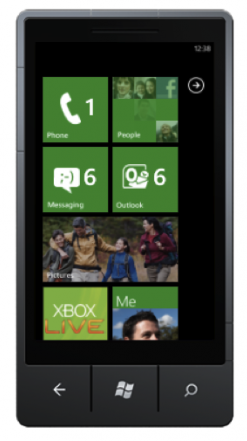
\includegraphics[scale=0.35]{images/WindowsPhone7.png}\\{Windows Phone 7}\\
\end{centering}


\subparagraaf{Other platforms}
% Onder other valt Symbian. Symbian is een app platforms dus we nemen het mee:)
\subparagraaf{Java ME}
\subparagraaf{Symbian}

\paragraaf{Distribution of applications}
%todo

\paragraaf{Market share and trend}
% TODO: waar de stats vandaan komen,  wat ze betekenen, waarom ik ze heb gekozen, wat de alternatieven zijn((gartner 2011)\
% platform specifiek maken: smartphone only? want daar focussen we op.

\begin{centering}
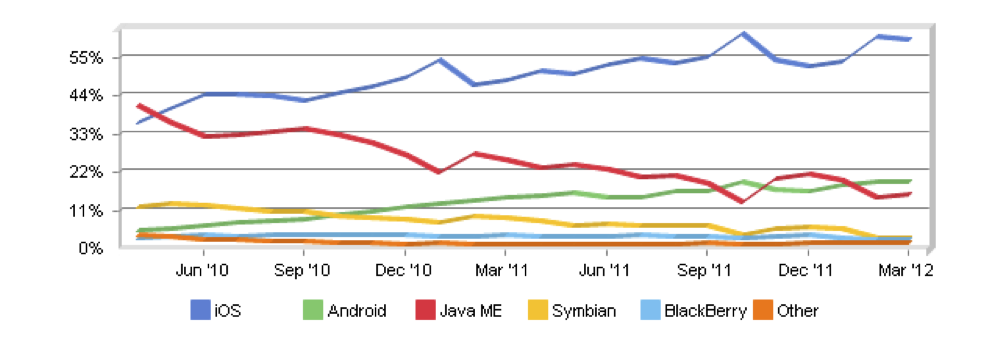
\includegraphics[scale=0.5]{images/marketsharetrendsApril10Tomay12.png}\\{World wide mobile OS Marketshare trends, April 2010 up to may 2012}\\
\end{centering}

\begin{centering}
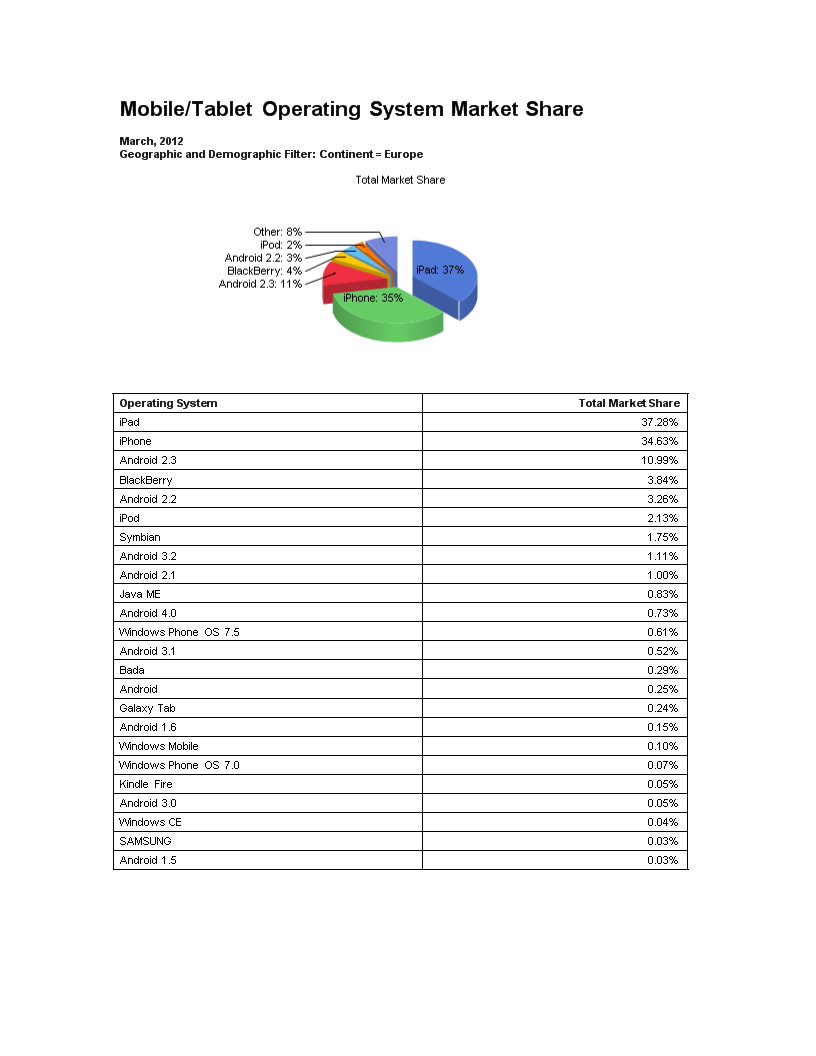
\includegraphics[scale=0.5]{images/netmarketshare_march2012.png}\\
\end{centering}

\begin{tabel}{|>\R p{\Procent{25}} | >\R p{\Procent{25}} |}{vbx}{Market share in the european continent as of march 2012\cite{Netmarketshare2012}}
\hline
\bf{Operating System} & \bf{Total \% Market Share}\\
\hline \hline
iOS & 74.04\\
Android & 18.36\\
BlackBerry & 3.84\\
Symbian & 1.75\\
Java ME & 0.83\\
Windows Phone & 0.68\\
Bada & 0.29\\
Windows Mobile & 0.14\\
Kindle & 0.05\\
Samsung & 0.03\\
LG & 0.01\\
ZTE & 0.00\\
Palm & 0.00\\
\hline
\end{tabel}

\paragraaf{Conclusion}
%vertellen waarom Android en iOS getarget worden: marketshare + trend koppelen aan een requirement van Lunatech


	\hoofdstuk{Defining native}
\paragraaf{Introduction}
This chapter will define the paradigm of \emph{native look-and-feel}.

\paragraaf{Native mobile applications}
A native application is an application inherent to the platform for which it was built using techniques proprietary to the platform. For example, an iOS application is native when written in Objective-C and an Android application is written in Java. Native applications are typically fast and can access the device's native API's.

\subparagraaf{The native look-and-feel}
When written in the native framework for a platform a mobile application receives acces to the available public libraries of the platform. These libraries include the UIKit\emph{(on iOS)} which provides the developer with a pre-fabricated set of user interface components. These can be seen as the building blocks for the graphical user interface on that platform. When used, the general style of the mobile application gains consitency to the overal user interface design of the platforms operating system. This gives an application its native look, which in turn participates to the \emph{native feel}.

%with a feeling of recognition when using the application, userinterface elements work as they expected based upon experience with using the operating system.
%todo: add some notes about the Human Interface Guidelines.

The \emph{native feel} of a mobile application can be defined as the speed in which the userinterface elements, the responsiveness of user interface elements to touch events, and smoothness of the animation in which the user interface elements are moved. A native mobile application has the advantage to hardware acceleration. This means its code has been precompiled and directly executed by the device CPU, rather than having to be interpreted by the device's browser. As a result of this the user interface elements are rendered faster and it \emph{feels} smooth.
 	

\paragraaf{Alternative mobile application types}
\subparagraaf{Web applications}
A mobile web application is an application developed with web technologies as JavaScript and HTML5 with CSS3. It is in fact nothing more than a website designed to fit on mobile devices, often they resemble the style of a native application rather than a traditional website. These applications are build with a JavaScript library to add support for scrolling and handling touch events. Touch events are handled via user interface elements provided by the library. Examples of these libraries include jQtouch, SenchaTouch.

% todo: screenshots/links neerzetten.

\subparagraaf{Hybrid applications}
A hybrid application in mobile development refers to an application which use a native shell to wrapped around web app. There are generally two forms of native shells, the first is a \emph{webview} and the second a native framework which exposes a javascript API to provide the web application access to otherwise native API's.

\subparagraaf{Webview-based hybrid applications}
A webview-based hybrid application is a webbased mobile application wrapped in a webview. A webview is a view or element which acts like a browser would, e.g. it is able to render HTML and run javascript.  It is readily available in the native libraries. The advantage of a webview-based hybrid application over an normal web application is that it can be published via the devices native application publishing platforms. e.g. a webview-based hybrid application targetted for the iPhone can be placed in the Apple appstore. 

Worklight is an example of a framework which can be used to develop webviewbased hybrid applications.

\subparagraaf{Framework hybrid applications}
A Framework based hybrid application is a webviewbased application build upon a framework which provides an API to allow the application access to otherwise native API's. The framework is written in the platforms native programming language making it possible to access the native API, such as reading contact list, composing of SMSes, full access to the location API, etc.

PhoneGap is an example of a framework which can be used to develop mixed hybrid applications.

\paragraaf{Comparison}
Web applications are quick and cheap to develop. Written entirely in HTML5, CSS and JavaScript. Executed by the mobile
browser and therefore cross - platform by default, but less powerful than native apps.
 
Hybrid Applications (Web), the app's source code consists of web code executed within a native wrapper that is provided by a framework.
 
Hybrid Applications (Mix), the developer augments the web code with a Javascript API to create unique features and
access native APIs that are not yet available via the browser, such as AR, NFC and others.
 
Native Application are platform-specific. Requires unique expertise and knowledge. Pricey and time consuming to develop but
 delivers the highest user experience of all approaches.

\begin{centering}
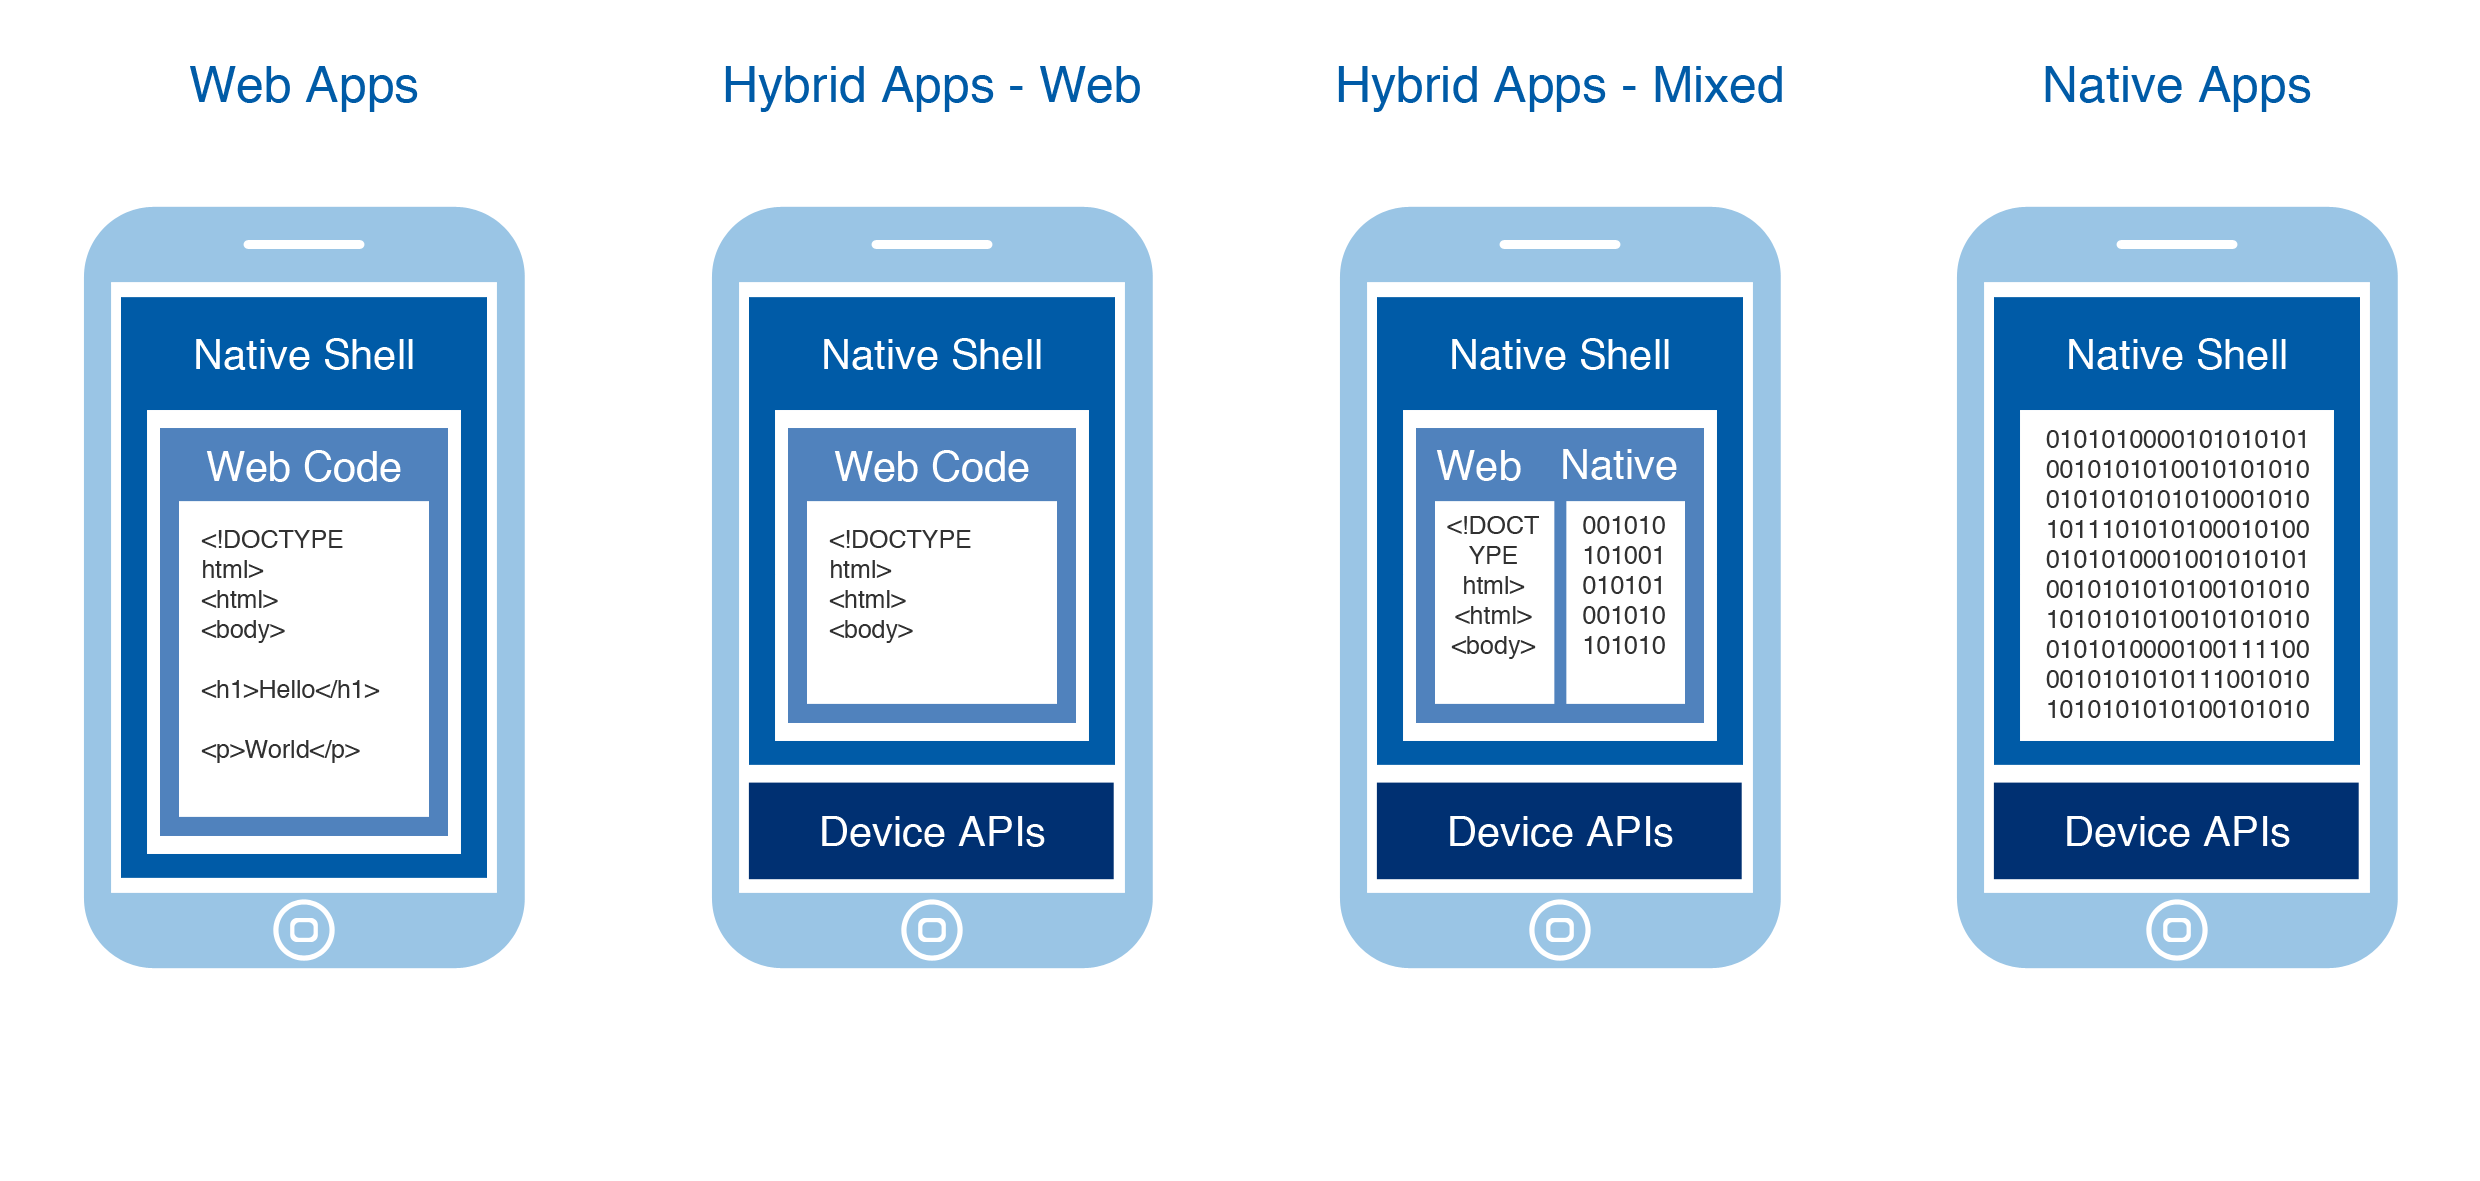
\includegraphics[scale=0.5]{images/apptypesdefined.png}\\{Different types of mobile applications\cite{IBM-Worklight2012}}\\
\end{centering}

\paragraaf{Conclusion}
A nativily written mobile application provides the user with an experience immersed to that of the level of the device's operationg system. This is due to two reasons:
\begin{itemize}
\item
\emph{Performance}\\
a native application is faster because it has direct access to memory and CPU
\item \emph{Looks}\\
a native application looks and feels more coherent to the device's operatingsystem because it is able to make use the of the provided userinterface elements.
\end{itemize}



	\hoofdstuk{Exsisting solutions to Cross-platform Mobile Application Development}
\paragraaf{Introduction}
In todays industry there exist several cross-platform mobile application development framework which offer a solution to cross-platform problem. All of these frameworks provide a custom solution for crossing the bridge between platforms. In order determine which one should be adopted by Lunatech for mobile development the following criteria have been determined for comparisson:

\begin{enumerate}
\item \emph{Platform support}\\
Which platforms and their versions are supported by the framework.
\item \emph{Native UI support}\\
Whether or not native user interface elements are supported for each supported platform.
\item \emph{Programming language}\\
Which programming language is used to develop using the framework.
\item \emph{IDE} (Intergrated Development Environment)\\
Which IDE can be used to develop using with the framework.
\item \emph{License type}\\
Which license types are available.
\item \emph{Application type}\\
Which type of mobile application is produced using this framework.
\end{enumerate}

The cross-platform criterium is based on Lunatechs requirement to build mobile applications for the operating systems have at least a 10 percent marketshare in the European continent. Second comes the support for native user interface elements. Together these criteria form the essence of the main research question: \emph{"How to develop a cross-platform mobile application while retaining the native look-and-feel?"}
The remaining criteria are of secondary importance, they will provide more detailed means to compare the frameworks which offer native user interface support.

The following solutions have been choosen for review: \emph{Titanium, Rhodes, Worklight and MoSync}. These are derived from the list Existing solutions\footnote{see attachment: \emph{Existing solutions}} this have been done based on by Lunatech provided requirements. %todo!

\paragraaf{Requirements}
%todo. - uitleggen waarom deze frameworks zijn geselecteerd.




\paragraaf{Appcelerator Titanium}
Appceleator Titanium is an commericially supported opensource platform for developing cross-platform mobile applications. It was introduced by Appcelerator Inc in December 2008. Built upon the Eclipse IDE Titanium offers a Javascript API to native proxy classes which allow the developer to generate truely native cross-platform mobile applications. 

\subparagraaf{Platform support and native capability}
As of may 2012 Titanium supports iOS and Android. Next to building a native application for these platforms Titanium offers the option to generate a web application. 
Support for Research in Motion (BlackBerry) is in active (however closed from public) development. May first 2012 Appcelerator announced that it is extending its core value of cross-platform native application development beyond iOS and Android, on to RIM's BlackBerry devices.\cite{Asher2012}

\subparagraaf{Techniques and tools}
TitaniumStudio is an Eclipse based IDE with integration the propriatory mobile SDKs and simulators. For iOS this means Titanium requires Xcode with the iOS SDK to be installed, for Android the Android SDK and the Android AVD\footnote{AVD: Android Virtual Device (device simulator)} are required.

Titanium applications are written in JavaScript but can be augmented with HTML \& CSS. During runtime the JavaScript is evaluated and executed via so-called \emph{proxy objects}.Proxy Objects are objects which are paired to a native object and can resemble native user interface elements.\footnote{Proxy objects are discussed in more detail in chapter x:Proxy objects \#TODO}.


\begin{centering}
	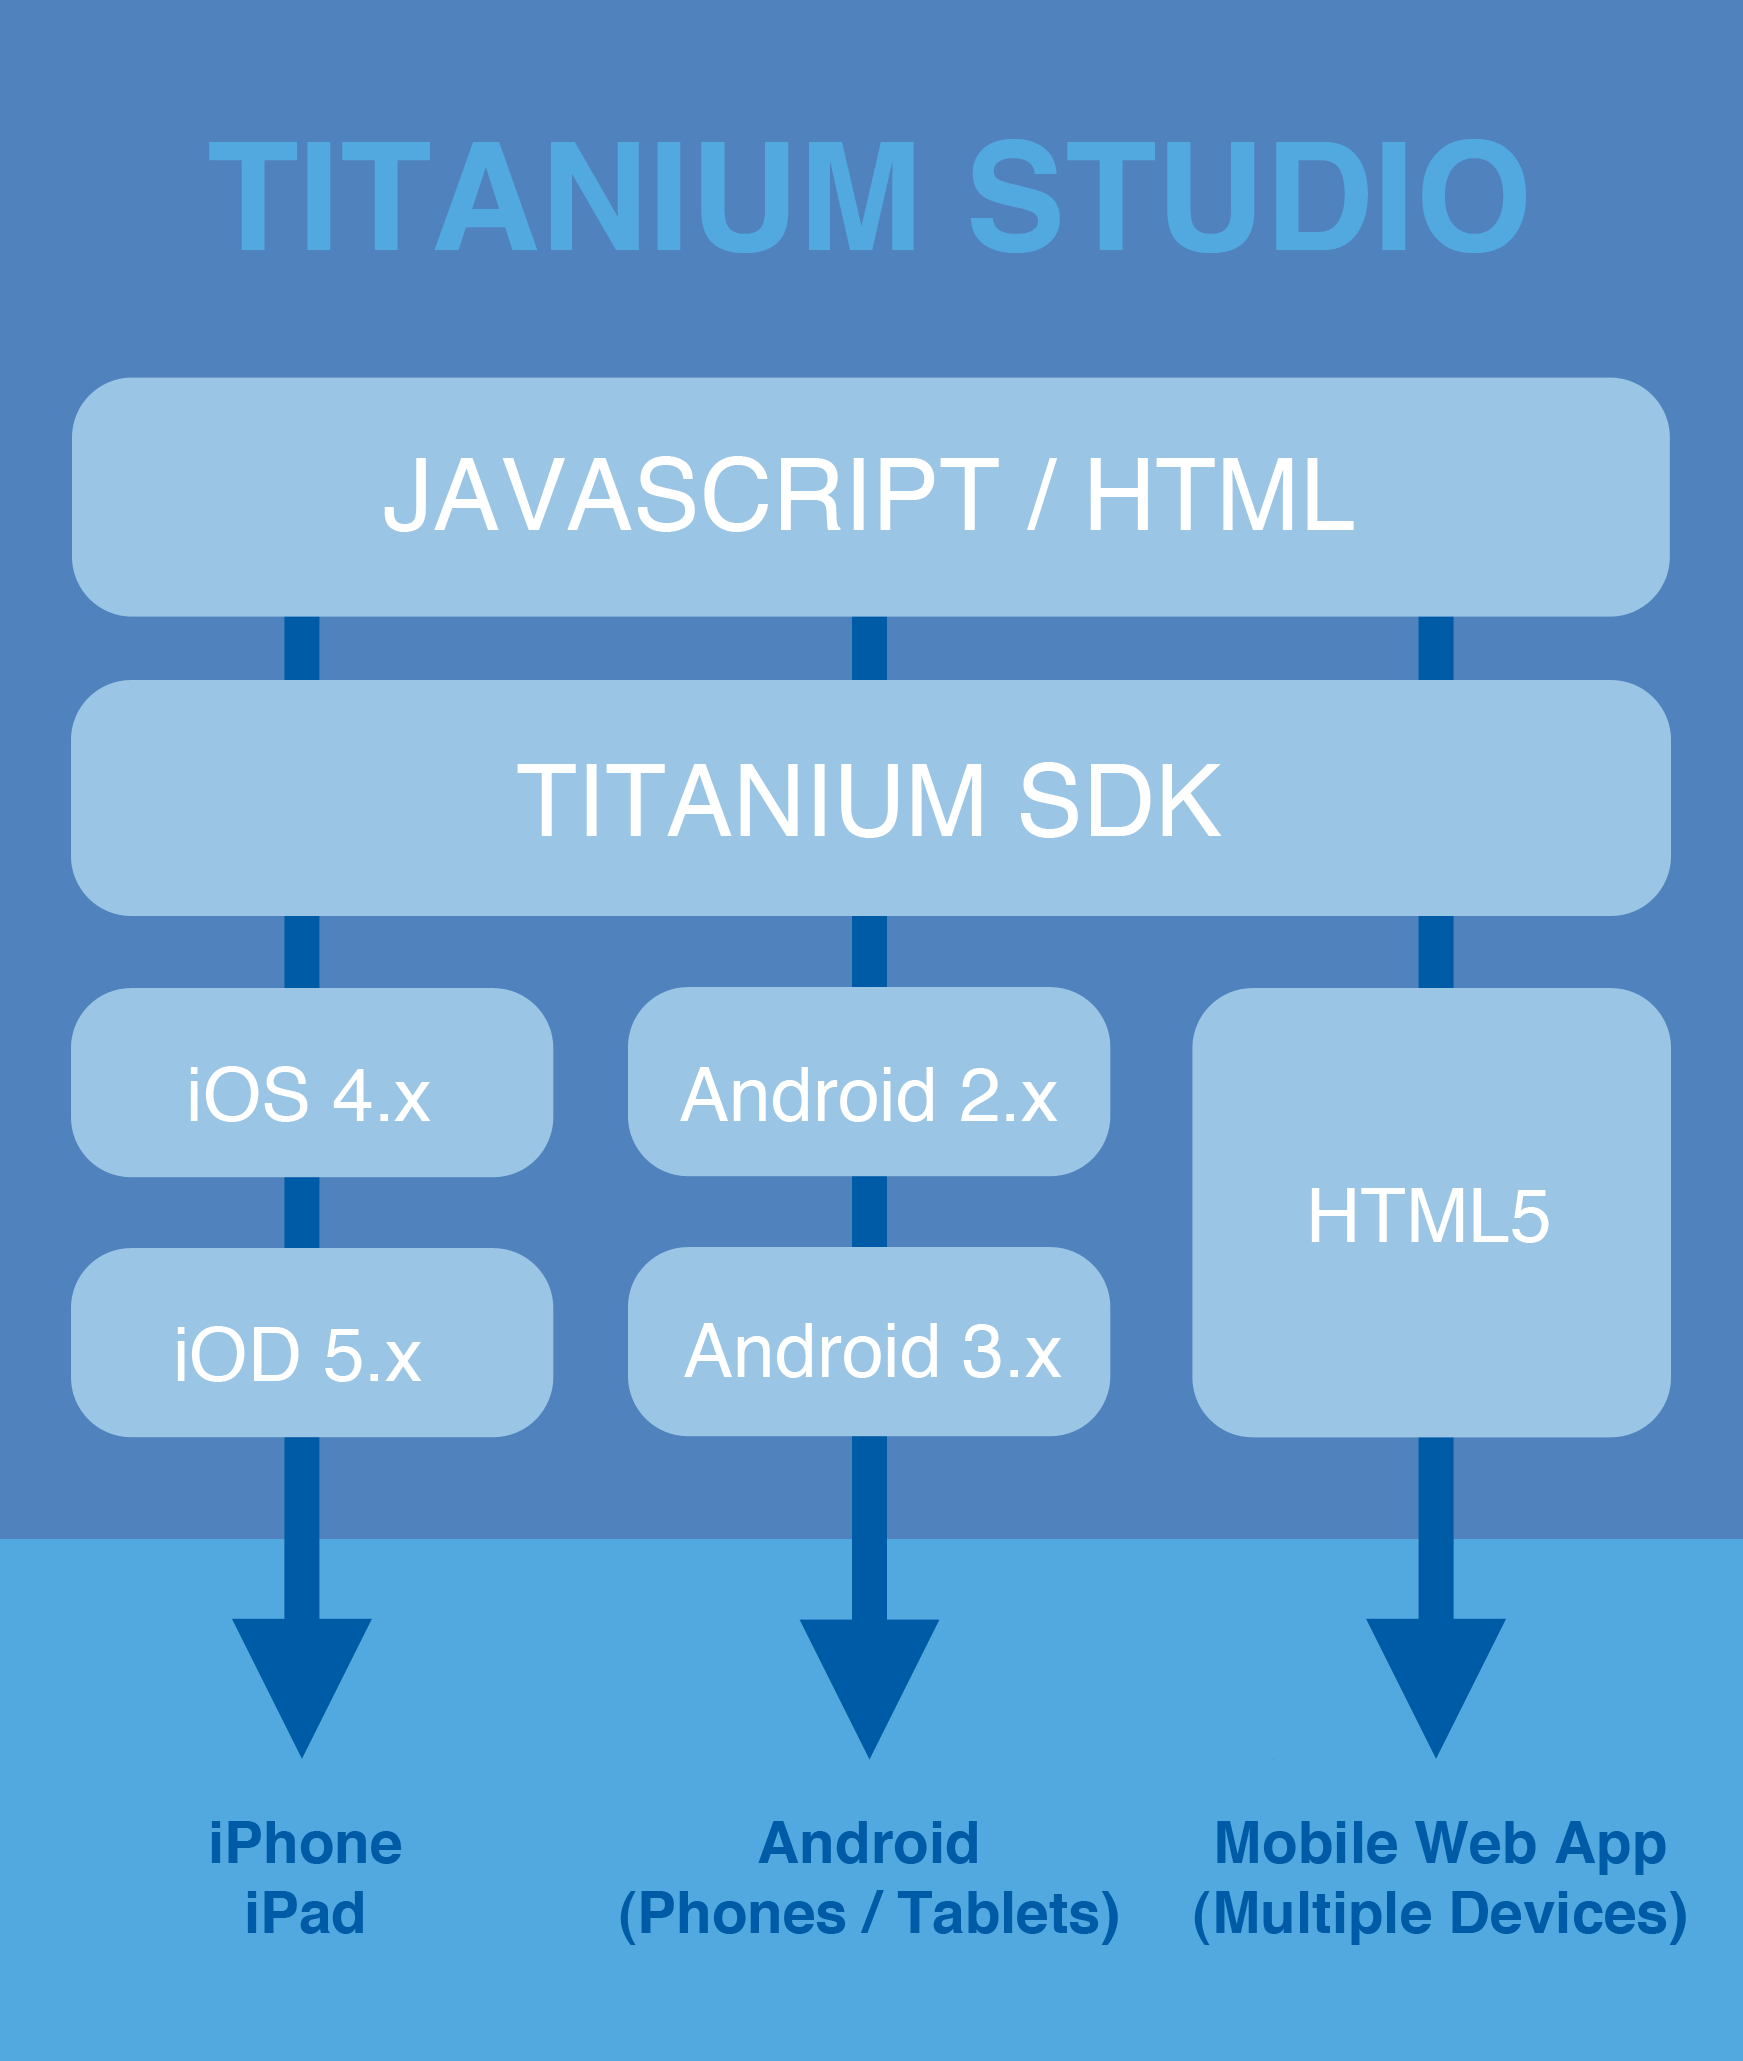
\includegraphics[scale=0.25]{images/titanium_architecture.png}\\{Titaniums bridge architecture\cite{Inc2012a}}\\
\end{centering}

\subparagraaf{Application type}
As mentioned above, Titanium applications are written in JavaScript but can be augmented with HTML \& CSS. The latter is in case a web application is required rather than a native application. This devices applications built with Titanium in two types:
\begin{itemize}
	\item
	Webapplications
	\item
	Native applications
\end{itemize}

\subparagraaf{Philosophy}
The goal of Titanium is to provide a high level, cross-platform JavaScript runtime and API for mobile development.\cite{Whinnery2012} Titanium aims to help developers levarage their JavaScript knowledge to build native mobile apps that run across multiple platforms.




\paragraaf{Rhodes}
Rhodes is an open source Ruby-based framework to build native applications for all major smartphone operating systems (iPhone, Android, RIM, Windows Mobile and Windows Phone 7). These are true native device applications (not mobile web applications) which work with synchronized local data and take advantage of device capabilities such as GPS, PIM contacts and calendar and the camera. %todo: herfomuleren

\subparagraaf{Platform support and native capability}
iOS, Android, BlackBerry, Symbian, Windows Mobile

\subparagraaf{Techniques and tools}
Eclipse based studio, Ruby \& HTML

\subparagraaf{Application type}
Even though Rhodes advertises producing fully native apps\cite{RhoMobile}, they do not. In fact all they do is provide the user with a framework, access to some navigational user interface controls, but the rest is a webview.
\begin{centering}
	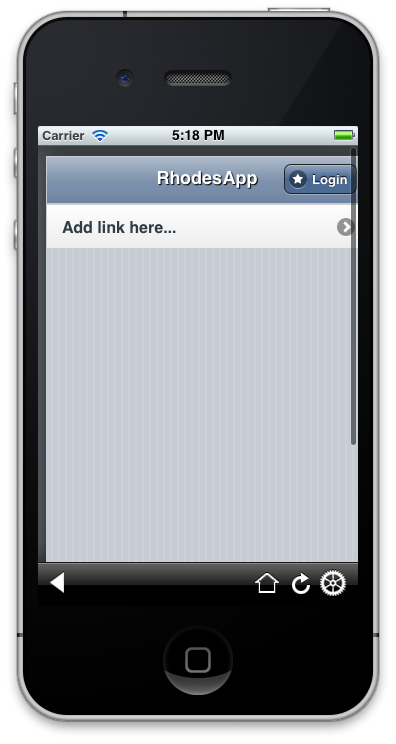
\includegraphics[scale=0.3]{images/rhodes_notsonative.png}\\{Rhodes sample iOS application: not fully native}\\
\end{centering}

\subparagraaf{Philosophy}




\paragraaf{Worklight}
Worklight Studio is an eclipse based IDE for the cross-platform development of mobile applications. Worklight Studio was introduced in 200x by Worklight Inc. In early 2012 Worklight Inc. became an IBM company. Worklight Studio offers mobile development trough the use of webtechnologies such as HTML5, and Javascript.

\subparagraaf{Platform support and native capability}
Worklight supports the following platforms: iOS, Android, BlackBerry and Windows Mobile 7.

\subparagraaf{Techniques and tools}
As mentioned above, Worklight Studio is an eclipse based IDE.
Allows the developer access to device APIs using native code or standard HTML5, CSS3 and JavaScript over a uniform PhoneGap bridge.


\subparagraaf{Application type}
Applications developed with Worklight can be classied as \emph{framework built hybrid applications}. As defined in the previous chapter this means the applications are based fitted inside webview and build on a framework which provides an API to allow the application access to otherwise native API's. The latter is achieved trough Worklights SDK while the former is made possible by an implementation of PhoneGap. \cite{Inc2012}

\begin{centering}
	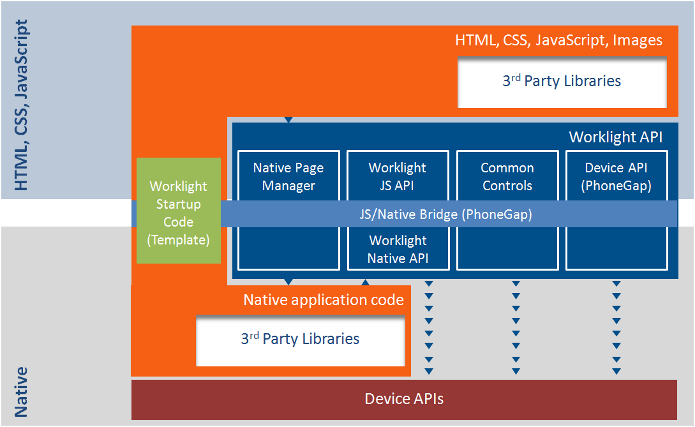
\includegraphics[scale=0.5]{images/Worklight_architecture.png}\\{Worklights bridge architecture\cite{Inc2012a}}\\
\end{centering}

\subparagraaf{Philosophy}
Worklight aims to grant developers access trough HTML5 to the capabilities that mobile devices provide. 


% Modern mobile users want on-the-go access to personalized data and context-driven services delivered at the right time and through the right channel. Augmented reality, Near Field Communication (NFC), push, geo-location, integration with cloud services, and mobile wallets are but a few of the current technologies that enable organizations to streamline operations, reduce costs and increase revenues.

% Worklight was designed from the ground up to address these exact needs. Built around HTML5, Worklight’s open approach does not employ proprietary translators, auto-compilers or esoteric coding languages. Our solution supports multiple development methodologies such as hybrid, web and native, which allow developers to access all of the unique capabilities that modern devices provide.


\paragraaf{MoSync}
The MoSync mobile SDK offers cross-platform development trough the use of webtechnologie or C/C++.

\subparagraaf{Platform support and native capability}

\subparagraaf{Techniques and tools}

\subparagraaf{Application type}

\subparagraaf{Philosophy}


\paragraaf{Comparisson} %todo..
	\hoofdstuk{Titanium analysis}

\paragraaf{Introduction}
Work in progress
%korte herhaling van wat titanium is, referentie naar existing solutions.
This chapter will analyze how Titanium works and why it provides the desired native \emph{look-and-feel}.
flexibility, extensibility

In this chapter we will attempt to analyze 

\paragraaf{Inner workings}

At runtime a mobile application developed with Titanium consists of three major components:
\begin{itemize}
	\item
	The JavaScript source code
	\item
	A platform-specific implementation of the Titanium API
	\item
	A JavaScript interpreter
\end{itemize}

During runtime the JavaScript source code will be integrated in a native class where it is encoded as a string and compiled. The implementation of the Titanium API done in a platform specific native programming language, Java for Android and Objective-C for iOS. The JavaScript interpreter evaluates the JavaScript code at runtime.


\subparagraaf{Runtime}
At runtime a JavaScript execution environment set up in the native environment, this is where the application source code is evaluated. Injected into JavaScript execution environment are so called \emph{proxy} objects.

\subparagraaf{Proxy objects}
A proxy object is an JavaScript object paired to an object in native code.\cite{Whinnery2012} This means the object exists in both JavaScript and native code. Proxy objects gap the bridge between the native and the JavaScript environment. A global Titanium object in JavaScript exposes access to the proxy objects. 

% So, for example var label = Titanium.UI.createTabel({ text: "label" }); will invoke a native method which creates a native UILabel object. 

% var b = Ti.UI.createButton({title:'Title'});, that will invoke a native method that will create a native UI object, and create a “proxy” object (b) which exposes properties and methods on the underlying native UI object to JavaScript.
% UI components (view proxies) can be arranged hierarchically to create complex user interfaces. Proxy objects which represent an interface to non-visual APIs (like filesystem I/O or database access) execute in native code, and synchronously (or asynchronously for APIs like network access) return a result to JavaScript. 


For example: In the JavaScript code, when a function is called on the global Titanium object to create a native UILabel a proxy object is created.
\   : voorbeeld afmaken
\begin{minted}[mathescape,
			   label="JavaScript-object",
               linenos,
               numbersep=5pt,
               gobble=0,
               frame=lines,
               framesep=2mm]{js}

var label = Titanium.UI.createTabel({
   text: "Lorem impsum",
   top: 10,
   left: 10,
   width: 100,
   height: 20
});
\end{minted}


In iOS the proxy button object:

\begin{minted}[linenos,
				label="Native-object",
				samepage,
				tabsize=2,
				xleftmargin=0cm,
               numbersep=5pt,
               frame=lines,
               framesep=2mm]{objc}
-(UILabel*)label
{
    if (label==nil)
    {
        label = [[UILabel alloc] initWithFrame:CGRectZero];
        label.backgroundColor = [UIColor clearColor];
        label.numberOfLines = 0;
        [self addSubview:label];
    }
    return label;
}
\end{minted}

\subparagraaf{JavaScript}
% %TODO verwoorden:
% JavaScript (sometimes abbreviated JS) is a prototype-based scripting language that is dynamic, weakly typed and has first-class functions. It is a multi-paradigm language, supporting object-oriented,[5] imperative, and functional[1][6] programming styles.
% JavaScript was formalized in the ECMAScript language standard and is primarily used in the form of client-side JavaScript, implemented as part of a Web browser in order to give enhanced user interfaces and dynamic websites. This enables programmatic access to computational objects within a host environment.
% JavaScript's use in applications outside Web pages — for example in PDF documents, site-specific browsers, and desktop widgets — is also significant. Newer and faster JavaScript VMs and frameworks built upon them (notably Node.js) have also increased the popularity of JavaScript for server-side web applications.
% JavaScript uses syntax influenced by that of C. JavaScript copies many names and naming conventions from Java, but the two languages are otherwise unrelated and have very different semantics. The key design principles within JavaScript are taken from the Self and Scheme programming languages.[7]


As mentioned above, Titanium uses JavaScript for cross-platform code compatibility. JavaScript is a logical choice because there are JavaScript Interpreters available for most platforms. This includes the targetted mobile platforms:

V8 is the default for Android but Rhino is also supported. V8 is has a better performance dealing as Rhino because it is directly intergrated to the NDK\footnote{Native Development Kit}. This means the code does not have to run trough the JVM\footnote{Java Virtual Machine}. Performance gain can exceed over 200\% processing time when parsing a JSON object.\cite{Lukasavage2011}
For iOS JavaScriptCore is the choosen interpreter.

These interpreters support the CommonJS specification.


\subparagraaf{CommonJS}
%TODO: verwoorden:
JavaScript is a powerful object oriented language with some of the fastest dynamic language interpreters around. The official JavaScript specification defines APIs for some objects that are useful for building browser-based applications. However, the spec does not define a standard library that is useful for building a broader range of applications.

The CommonJS API will fill that gap by defining APIs that handle many common application needs, ultimately providing a standard library as rich as those of Python, Ruby and Java. The intention is that an application developer will be able to write an application using the CommonJS APIs and then run that application across different JavaScript interpreters and host environments. With CommonJS-compliant systems, you can use JavaScript to write:

Server-side JavaScript applications
Command line tools
Desktop GUI-based applications
Hybrid applications (Titanium, Adobe AIR)



\subparagraaf{Modules}
%TODO: verwoorden:
By default, JavaScript runs programs in a global scope and doesn't have any native namespacing language features. This means that, unless you're careful, your programs can descend into a mess of code spaghetti, full of conflicting variables and namespace pollution.

CommonJS modules are one of the best solutions to JavaScript dependency management.

CommonJS modules solve JavaScript scope issues by making sure each module is executed in its own namespace. Modules have to explicitly export variables they want to expose to other modules, and explicitly import other modules; in other words, there's no global namespace.

Modules prevent variables from glogging up the global namespace.


a sample module:


\begin{minted}[mathescape,
         label="eventCell.js",
               linenos,
               numbersep=5pt,
               gobble=0,
               frame=lines,
               framesep=2mm]{js}
function eventCell(Event, delegate) {
  // cell code removed
  return this.cell;
};
module.exports = eventCell;
\end{minted}

Is used like:
\begin{minted}[mathescape,
         label="eventCell.js",
               linenos,
               numbersep=5pt,
               gobble=0,
               frame=lines,
               framesep=2mm]{js}
  var messageCell = require('stager/tableview/messageCell');
  tableview.appendRow(new messageCell(message, that));
\end{minted}

% gaat er te ver op in:
% \paragraaf{Eclipse}
% \paragraaf{Buildsystem}
% \paragraaf{XCode CLI and the iOS SDK}
% \paragraaf{Android SDK}

\paragraaf{Usage concepts}
\subparagraaf{Window Navigation}
\subparagraaf{View hierarchie}
\subparagraaf{Event handling}

\paragraaf{Extensibility and flexibility}
\subparagraaf{Module system}

\paragraaf{Performance versus flexibility}
tableview.

\paragraaf{Documentation}
all in one place
wide range: video tutorials to confluence based guides


\paragraaf{Summary}
% werking, architectuur, kort samenvatten
Titanium provides the \emph{native look-and-feel} trough proxy objects. 

	\hoofdstuk{Case study}

\paragraaf{Introduction}
Mobile application has been developed with Titanium to study its flexibility and features.


\paragraaf{Stager}
In 2011, live music venue WORM hired Lunatech to build \emph{Stager}, a modern web-based resource planning and ticketing application to help manage live music events. Lunatech took the opportunity to use the relatively new Play framework to build a web application with an HTML5 and Java architecture. Stager has broad requirements ranging from high performance and security for the public ticket sales component to high usability for the internal resource planning component that will be used for hours a day by employees and being open to enhancements in the future for new customers. \cite{Lunatech2011}

\subparagraaf{WORM}
WORM is an institute for avantgardistic recreation Rotterdam, consisting of an artistscollective, a podium with a bar and Parallel University (DIY workshops for film, music and media). Born under the stars of punk, Dada, Fluxus, Situationism and futurism WORM is grown into a headstrong organization that the 'Do-It-Yourself' mentality of their ancestors, combined with ultra-pragmatism, love of technique (s) and proper accounting. Worm outputs film, radio, concerts, courses, partys, publications, performances, web projects, installations, workshops and an accumulation of tactile media and internet.WORM focuses (cheerful yet serious) in avantgarde, resource scarcity and opensource. \cite{WORM2012}

\paragraaf{Stager app}
As described in the chapter \emph{Background} Stager is an planning and ticketing application to help manage live music events. In addition to planning and ticketing Stager features an \emph{atomfeed} to publish events. A Stager app would make use of this atomfeed to list any published events on a mobile device.


\paragraaf{Stager application requirements}

List of current and upcoming events
events are downloaded in JSON format from the Stager event atomfeed at /web/feeds/events
events are displayed in a row-based layout
events are linked to their corresponding event detailview
events in the list are sorted by date (asc)
events in the list contain labels with event title, subtitle, date

Detailview of an event
Shows detailed event information of an selected event:
event title, 
subtitle, 
date, 
times (doors open, start, end), 
location details (venue name, street, number, city), 
event content (html rendered text)

Add event to agenda
Prompts the user: "Add event 'x' on date 'y' in agenda?"
Adds a selected event to the mobile devices agenda.
Prompts the user of succes of add action.

Start gps-based navigation towards physical location of event
Prompts the user "Navigate to y?" (y in the format of: streetname, housenumber, cityname, postalcode)
Opens map application with address as argument.

View media attached to an event
Media defined as: URL's to event images, videos, websites.

Display in a grid or list, categorize media types.
Each displayed media item is resembled by a tumbnail or icon.
When selected a media item opens to its content in:
images an included webview,
websites the device browser,
for videos the youtube app or the browser( depending on video type \& location).

Share event details to social media
An event detail view will contain a 'share/deel' button.
Prompts the user for platform to share. (twitter/facebook/email)
Default value (editable): "I am attending event x on date y in location x !"

	
(Un)Register device to receive push notifications on new events of interest
Register the device to receive pushed notifications about upcoming events which might be of interest to the user.
Based on Relation.interest model in Stager.



\subparagraaf{Events}



\subparagraaf{Notifications}
\subparagraaf{Tickets}
\subparagraaf{i18n}
\subparagraaf{Mobile payment}
\paragraaf{Used techniques and methodologies}
\subparagraaf{Javascript}
For Titanium Javascript is the only option. Everything that can be written in JavaScript will eventually be written in JavaScript.
\subparagraaf{CommonJS}
\subparagraaf{Playframework}
\subparagraaf{Java}
\subparagraaf{JSON}
%\paragraaf{Titanium modules}
%\paragraaf{Stager service modules}


\paragraaf{Conclusion}
%Samenvatten wat er gedaan is aan de Stager app, welke platforms het draaid, e.d.
	\hoofdstuk{Conclusion and Recommendations}
% With Appcelerator Titanium one is able to develop cross-platform mobile applications while retaining the native look at feel.

% There are serveral solutions to crossplatform mobile development. However due to the high bar set to what Lunatech defines as native only Titanium is a possibility.


\paragraaf{Main research goals}

\begin{shadequote}
Titanium is a commercially viable solution to the cross-platform development of mobile applications%\par\emph{W. de Kraker, 2012}
\end{shadequote}


\paragraaf{Stager case study}

\paragraaf{Cross-platform Mobile Application Development using Titanium}


\paragraaf{Project goals}



\subparagraaf{Evaluation of Titanium}

\subparagraaf{Limitations of Titanium}

\paragraaf{Recommendation}
% - If the current native look and feel definition is not changed
% Yes, Titanium should be considered a development platform. 
\ifpublic
% todo.
%	\iflanguage{dutch}{\def\bibname{\normalsize{Bronnen}}}
%		{\def\bibname{\normalsize{References}}}
%	{\footnotesize{\input{bronnen}}} 
\else
	\bibliographystyle{plain}
	\bibliography{bibliography}
	\hoofdstuk{Evaluatie}
	\appendix
	%\include{attachment} 
\fi
\end{document} 